Pentru a putea interpreta datele rezultate le-am clasificat manual în tabel la fel ca și cele de obținute folosind alpha-beta-CROWN. Câmpurile de tabel sunt identice cu cele de la alpha-beta-CROWN, singura excepție fiind ocurența a două noi timpuri de rezultate, și anume:
\begin{itemize}
    \item \textbf{results (vnncomp2023/us)}: Poate avea valori sat/unsat/unknown/error; pentru \textbf{sat} și \textbf{unsat} interpretările sunt la fel ca și în cazul alpha-beta-CROWN, pentru \textbf{unknown} înseamnă că proprietatea nu a putut fi demonstrată, iar \textbf{error} rezultă atunci când a avut loc o eroare în timpul rulării tool-ului.
    Prima coloană cu rezultate reprezintă rezultatele obținute în competiție, iar a două coloană cu rezultate este obținută de noi.
\end{itemize}

În tabelul de mai jos se prezintă o analiză comparativă între rezultatele obținute în urma rulării proprii și cele obținute în cadrul competiției.

\begin{figure}[h]
\centering 
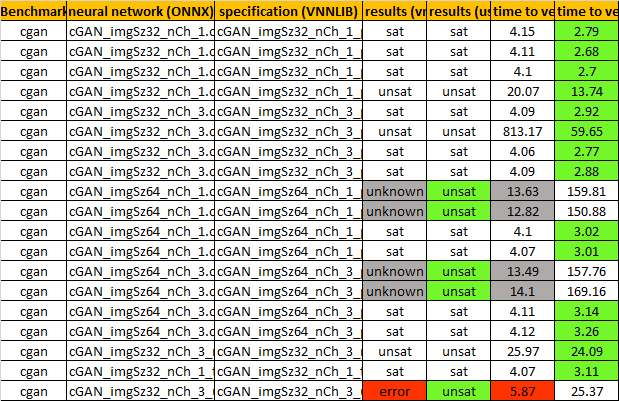
\includegraphics[width=0.8\linewidth]{imagini/interpretare rezultate/NeuralSAT_comp_vs_us.png}
\caption{Comparare rezultate NeuralSAT}
\label{fig:image2} 
\end{figure}
\

Conform tabelului prezentat în \ref{fig:image2}

Graficul prezentat mai jos, evidențiază și mai mult distribuirea timpilor de execuție pentru fiecare instanță în parte.